\section{Lösungsidee}
\begin{wrapfigure}{r}{0.45\textwidth}
	\setlength\intextsep{0pt}
	\centering	
	\includegraphics[width=0.4\textwidth]{Grafiken/sek3abb1}
	\caption{Verbesserte Bilderkennung}
	\label{abb:transform}
\end{wrapfigure}
Die in Kapitel 1 vorgestellte Einleseprozedur wird den Anforderungen für die Erkennung eines Fotos oder eines Scans nicht gerecht. Bei schwankender Ausleuchtung des Bildes lässt sich kein geeigneter Schwellwert bestimmen. Stattdessen wende ich verschiedene Algorithmen des maschinellen Sehens an, um ein möglichst ideales Bild aus dem Eingabebild zu extrahieren.

Ich extrahiere zunächst alle Kanten des Bildes. Kanten sind Stellen, an denen sich die Farbwerte eines Pixels schlagartig ändern. Den Kantenextraktionsalgorithmus implementiere ich hierbei so, dass die Kante eine lückenlose Linie darstellt.

Mit diesen Kanten habe ich das Bild segmentiert. Zu schwärzende Bildsegmente sind von einer Kante umrandet. Daher fülle ich jedes Segment komplett schwarz (1), während ich den Hintergrund weiß (0) belasse.

Die Färbung basiert auf die folgende Annahme: Der Hintergrund des Bildes ist monoton gleichfarbig. Alle an den Hintergrund angrenzenden Segmente sind Bestandteile eines Kreisringes. Schließlich fand dort eine schlagartige Farbänderung zum Hintergrund statt. Die Felder, die an diese Segmente angrenzen, sind weiß, da sich die Farbe wiederum schlagartig zum Hintergrund zurück geändert hat. Dieses Muster setze ich fort, bis die Farben aller Segmente bestimmt sind.

Die drei Schritte der Bildprozessierung sind in Abbildung \ref{abb:transform} dargestellt.

Vorteil dieser Vorgehensweise gegenüber einem Schwellwertverfahren ist, dass jeder ähnlich gefärbte Bereich durchgehend gleich gefärbt wird. Bei einem Schwellwertverfahren werden bei einem zu kleinen Schwellwert dunklere Bildbereiche komplett geschwärzt, während bei einem zu hohen Schwellwert einige Kreis-Codes nur lückenhaft erkannt werden.
 
\section{Umsetzung}
\subsection{Graustufenbild}
In einem ersten Schritt ermittle ich aus dem farbigen Bild ein Graustufenbild. Dies erfolgt mit einer gewichteten Mittlung aus den Intensitätswerten der drei Primärfarbkanäle. Laut der Norm CIE 1931\footnote{\url{en.wikipedia.org/wiki/Grayscale}} ist der Grauwert mit folgender Formel zu bestimmen:

\begin{equation}
Y = 0,2126R+0,7152G+0,0722G
\end{equation}

\subsection{Canny-Edge-Detector}
Um in diesem Graustufenbild die Kanten zu bestimmen, nutze ich den 1986 von John Canny vorgestellten Canny Edge Detector. Zu diesem habe ich mich auf einer Online-Veröffentlichung der Universität von Edinburgh informiert: \url{http://homepages.inf.ed.ac.uk/rbf/HIPR2/canny.htm} Dort finden Sie weitere Erläuterungen zu dem Canny-Edge-Detector, den ich im folgenden kurz darstelle.

\subsubsection{Weichzeichnung (Listing \ref{lst:gauss})}
In einem ersten Schritt filtere ich vor der eigentlichen Kantenerkennung grobe Ausreißer aus dem Bild heraus. Hierfür wende ich einen Gaußschen Weichzeichner an. Ein solcher Weichzeichner funktioniert, indem für jedes Pixel ein gewichteter Mittelwert aus seinem eigenen Grauwert und den Grauwerten seiner Umgebung bestimmt wird. Der Gewichtung wird die Gaußsche Normalverteilung zugrunde gelegt. Ich habe mich für ein Sigma von 3 entschieden. So werden grobe Ausreißer entfernt, der Kantenverlauf bleibt jedoch erhalten. Aus dieser Kurve lässt sich folgende Matrix extrahieren\footnote{\url{http://dev.theomader.com/gaussian-kernel-calculator/}}:
\begin{equation}
	\begin{bmatrix}
	0,031827&0,037541&0,039665&0,037541&0,031827 \\
	0,037541&0,044281&0,046787&0,044281&0,037541 \\
	0,039665&0,046787&0,049434&0,046787&0,039665 \\
	0,037541&0,044281&0,046787&0,044281&0,037541 \\
	0,031827&0,037541&0,039665&0,037541&0,031827 \\
	\end{bmatrix}
\end{equation}
Jeder Pixel wird mit dem mittleren Wert multipliziert. Die umliegenden Pixel werden mit ihren Pendants in der Matrix multipliziert. Die Summe aus allen Produkten entspricht dem neuen Wert des Pixels.

Allerdings kann die Gaußsche Weichzeichnung auch in einen horizontalen und vertikalen Bestandteil aufgeteilt werden. Nach dieser Aufteilung erhält man folgende Matrix:
\begin{equation}
	\begin{bmatrix}
	0,1784&0,210431&0,222338&0,210431&0,1784
	\end{bmatrix}
\end{equation}
Man kann mit dieser Matrix das gleiche Ergebnis erzielen, indem man sie zunächst in horizontale und anschließend in vertikale Richtung anwendet. Diese Vorgehensweise hat eine bessere Laufzeit, da für die Glättung eines Pixels nicht \(4^2\), sondern nur \(2\times 4\) Pixel betrachtet werden müssen.

\subsubsection{Sobel-Operator (Listing \ref{lst:sobel})}
Anschließend wende ich auf das nun geglättete Bild den Sobel-Operator an. Dieser Operator entspricht der 1. Ableitung über die Helligkeitskurve des Bildes. Der Operator wird mithilfe von \textit{Convolution} über das gesamte Bild berechnet. Convolution ist das bereits von dem Gauß-Weichzeichner bekannte Prinzip, das auf jedes Pixel eine Matrix angewandt wird. Der Sobel-Operator basiert auf zwei Convulution-Durchläufen mit folgenden Matrizen:
\begin{gather}
	\begin{split}
		\begin{bmatrix}
			-1,0&-2,0&-1,0\\
			0,0&0,0&0,0\\
			1,0&2,0&1,0\\
		\end{bmatrix}
	\end{split}
	\hspace{5em}
	\begin{split}
		\begin{bmatrix}
			-1,0&0,0&1,0\\
			-2,0&0,0&2,0\\
			-1,0&0,0&1,0\\
		\end{bmatrix}
	\end{split}
\end{gather}

Diese Matrizen entsprechen der Ableitung in vertikale und horizontale Richtung, da die jeweils an das Feld in horizontale oder vertikale Richtungen angrenzenden Felder voneinander subtrahiert werden.
Wenn die umliegenden Pixel den gleichen Intensitätswert haben, ist das Ergebnis des Sobel-Operators 0.
Bei Intensitätsunterschieden verändert sich das Ergebnis des Operators entsprechend.
Da allerdings für die weiteren Berechnungen eine kombinierte Ableitung benötigt wird, müssen beide Ableitungswerte eines Pixels kombiniert werden.

Hierfür können die beiden Ableitungswerte als ein rechtwinkliges Dreieck aufgefasst werden. Die Ausschläge der Ableitungen in x- und y-Richtung entsprechen den beiden Katheten. Ein kombinierter Wert aus beiden Ableitungen entspricht dann der Länge der Hypotenuse. Diese lässt sich mit dem Satz des Pythagoras berechnen (\(G_{xy} = \sqrt{G_x^2 + G_y^2}\)).

\subsubsection{Non-Maximum-Supression (Nichtmaximumsunterdrückung) (Ebenfalls Listing \ref{lst:sobel})}
Leider liefert der Sobel-Operator Kanten, die mehrere Pixel breit sind. Schließlich verlaufen die Kanten in einem Foto nicht vollkommen abrupt, sondern verlaufen über mehrere Pixel. 
Ein Lösungsansatz zur Berechnung von möglichst dünnen Kanten ist die Nichtmaximumsunterdrückung (NMS). 

Da die beiden Ableitungsfunktionen ein rechtwinkliges Dreieck bilden, kann mithilfe der Tangensfunktion der Winkel der Kante ermittelt werden:
\begin{equation}
	tan(\alpha) = \frac{G_y}{G_x}
\end{equation}

Mit diesem Winkel können die Pixel bestimmt werden, die an der gleichen Kante liegen. Wenn der Ableitungswert des Pixels nicht das Maximum seiner Nachbarn darstellt, kann sein Ableitungswert auf 0 gesetzt werden (Der Pixel wird in der Ausgabegrafik unterdrückt). Schließlich gibt es entlang der Kante einen stärken Farbintensitätsunterschied.  

Wenn der Winkel beispielsweise \(0^{\circ}\) beträgt, verläuft die Kante in horizontale Richtung. Dann wird der Ableitungswert des Pixels mit seinem nördlichen und südlichen Nachbarn verglichen.
Nur wenn der Ableitungswert das Maximum von diesen Pixeln darstellt, ist er Teil der 1px breiten Kante. Sonst ändert sich bei diesem Pixel zwar die Farbe. Aber es folgt unmittelbar ein noch stärkerer Farbumschlag.

\subsubsection{Binärisierung mit Hysterese (Listing \ref{lst:hyst})}
Zur Binärisierung des Ergebnisses der Sobel-Operators wende ich eine Technik namens \textit{Hysterese} an. Bei einer Hysterese wird zunächst mit einem hohen Schwellwert das Bild binärisiert. 
Im Kontext meiner Implementierung bedeutet dies, dass alle Pixel mit einem Ableitungswert höher als 40 im Ausgabebild der Canny-Eckenerkennung schwarz gefärbt werden.

Da aber möglicherweise eine Kante auch aus weniger stark abgesetzten Pixeln besteht, akzeptiert die Hysterese für an bereits erkannte Kantenpunkte anliegende Punkte einen niedrigeren Schwellwert. Sobald ein Punkt einer Ecke gefunden wurde, wird diese "`verfolgt"'.

Diese Verfolgung ist mit einem Stack implementiert. Jeder im Erkennungsschritt mit hohem Schwellwert erkannte Pixel wird auf diesen Stack gelegt. Nach Abschluss des Erkennungsschrittes werden alle Pixel, die an ein Pixel aus dem Stack angrenzen, noch nicht gefunden wurden und über dem verringerten Schwellwert von 1 liegen, schwarz markiert. Diese Pixel werden wiederum auf den Stack gelegt, sodass die Kante mit dem verringerten Schwellwert verfolgt wird. 

\subsubsection{Dilation (Listing \ref{lst:dilation})}
Aufgrund der Non-Maximum-Supression sind kleine Lücken in der Grafik entstanden. Dies verhindert eine sinnvolle Ausführung von den in meinem Algorithmus häufig verwendeten Flood-Fills. Daher wende ich auf das Ergebnis der Hysterese Dilation an. Hierbei wird jedes Pixel, das mehr als einen schwarzen Nachbarn hat, geschwärzt.
Damit verdicke ich die Linie. Allerdings ist sie weiterhin weitaus exakter, als sie es ohne Non-Maximum-Supression wäre.

\subsection{Einfärben des Bildes (Listing \ref{lst:ausf})}
Der Canny-Detektor gibt ein Bild aus Kanten aus (Mittlere Grafik in Abb. \ref{abb:transform}). Die weiteren Berechnungsschritte benötigen jedoch ein Bild, in dem der Kreis, der Kreisring und die Segmente komplett schwarz eingefärbt sind. Unter Ausnutzung der Annahme aus der Lösungsidee habe ich einen Algorithmus formuliert.
Dieser nimmt als Eingabe das Ergebnis des Canny-Eckenerkennungsprozesses und hat als Ausgabe ein Binärbild als boolesches 2D-Array. Damit ist das Ausgabeformat der neuen Bildeinleseprozedur identisch zu dem der simplen Einleseprozedur aus Kapitel 1.

Von Pixel(0|0) ausgehend werden alle im Canny-Bild erreichbaren weißen Pixel mithilfe einer Flood-Fill im Ausgabebild als weiß abgespeichert, da diese den Hintergrund darstellen.

Anschließend werden alle Kantenpixel, die an den Hintergrund angrenzen, schwarz markiert. Diese Pixel stellen eine Kante zum Vordergrundbereich dar.
Da sie die Kante zum Vordergrundbereich sind, werden alle an diese Pixel angrenzenden Nicht-Kanten-Pixel, die im Ausgabebild noch nicht markiert wurden, schwarz markiert. Schließlich befindet sich dieser Bereich weiterhin im Vordergrund.
Diese Prozedur wird abwechselnd zur Bestimmung von Vorder- und Hintergrundbereichen eingesetzt.

Praktisch umgesetzt habe ich dies mit einer Entlehnung aus der Graphentheorie.\footnote{\url{https://en.wikipedia.org/wiki/Connected-component_labeling}}. Mein Algorithmus basiert auf der im Abschnitt "`One component at a time"' vorgestellten Idee.

In einem Integer-Array gebe ich jedem Hintergrundpixel den Wert 0. Darauf gebe ich den anliegenden True-Pixeln den Wert 1. Die an diese Kante anliegenden False-Pixel erhalten ebenfalls den Wert 1, da sie wie oben geschildert zu der Kante gehören.

Danach fahre ich mit der nächsten Kantengruppe fort, nur vergebe ich dort den Wert 2. Schlussendlich müssen dann Pixel mit einem ungeraden Wert schwarz gefärbt werden, während Pixel mit einem geraden Wert weiß belassen werden.

\subsection {Rotation der Kreis-Codes (Listing \ref{lst:decode})}
In einem Foto ist nicht davon auszugehen, dass der Nutzer das erste Segment exakt an der x-Achse ausrichtet. Daher muss der Trapezkranz aus Kapitel 2 so über den Kreisring gelegt werden, dass jedes Trapez möglich exakt über einem Kreisringsegment liegt. 

Dies gelingt, indem die Achse so verschoben wird, dass sie auf einer Kante zwischen zwei Kreisringsegmenten liegt. Dafür muss eine beliebige Kante auf dem äußeren Kreisring gefunden werden. An einer solchen Stelle muss in einem Abstand von \(4,7u\) vom Pol (vgl. Abb. \ref{abb:dims}) eine Kante vorliegen. Also muss an dieser Stelle im Ausgabebild von Canny True stehen. Zu beachten ist, dass hier nicht das ausgefüllte Bild genommen werden darf, da nach Kanten, nicht nach Segmenten, gesucht wird.
So suche ich in jedem Winkel vom Pol aus eine Kante.

Dann addiere ich den Winkel \(0^{\circ} \le \delta \le 360^{\circ}\) zwischen der x-Achse und dem Strahl zu einer beliebigen Kante auf jeden der einteilenden Strahlwinkel hinauf. Somit verschiebe ich den gesamten Trapezkranz so, dass er exakt auf den Trapezen liegt. Statt den Formeln \ref{eq:nKoords} nutze ich folgende Formeln:

\begin{gather}
	\begin{split}
		x_1 &= cos(n \cdot \frac{22,5\pi}{180} + \delta) \cdot 5,5u + x_0\\
		y_1 &= sin(n \cdot \frac{22,5\pi}{180} + \delta) \cdot 5,5u + y_0\\ \vspace{2em}
		x_2 &= cos(n \cdot \frac{22,5\pi}{180} + \delta) \cdot 4,5u + x_0\\
		y_2 &= sin(n \cdot \frac{22,5\pi}{180} + \delta) \cdot 4,5u + y_0
	\end{split}
	\hspace{1.2em}
	\begin{split}
		x_3 &= cos(((n+1)\bmod{}16) \cdot \frac{22,5\pi}{180} + \delta) \cdot 5,5u + x_0\\
		y_3 &= sin(((n+1)\bmod{}16) \cdot \frac{22,5\pi}{180} + \delta) \cdot 5,5u + y_0 \\ \vspace{2em}
		x_4 &= cos(((n+1)\bmod{}16) \cdot \frac{22,5\pi}{180} + \delta) \cdot 4,5u + x_0\\
		y_4 &= sin(((n+1)\bmod{}16) \cdot \frac{22,5\pi}{180} + \delta) \cdot 4,5u + y_0
	\end{split} \label{eq:nKoordsNeu}
\end{gather}

Dass dadurch mehr als \(360^{\circ}\) in den Sinus eingegeben werden ist unwesentlich, da sich die Sinuskurve nach \(360^{\circ}\) wiederholt.
\pagebreak
\section{Beispiele}
Allen Optimierungen zum Trotz erkennt mein Programm in den weiteren Beispielen nicht alle Kreis-Codes. Ausgabebilder aller BwInf-Beispiele finden Sie in der Einsendung. Hier gebe ich tabellarisch wieder, wie vollständig das Programm die Beispieleingaben dekodiert hat. \\ 
(\checkmark{} Vollständig, \(\varnothing\) unvollständig, \(\times\) ohne Ergebnis)

\begin{table}[!h]
    \begin{tabular}{lllllllllll}
    Cam 1             & Cam 2           & Cam 3           & Cam 4             & Cam 5           & Cam 6           & Cam 7           & Cam 8             & Cam 9           & Cam A           & Cam B      \\ \hline
    \(\varnothing\) & \checkmark & \checkmark & \(\varnothing\) & \checkmark & \checkmark & \checkmark & \(\varnothing\) & \checkmark & \checkmark & \(\varnothing\)\\
    \end{tabular} \\ \\
    \begin{tabular}{lllllll}
    Bitmap & Noise 25      & Noise 50      & ROT         & CMYK        & Grey (GIF)  & Grey (JPG)  \\ \hline
    \checkmark & \checkmark & \(\times\) & \checkmark & \checkmark & \checkmark & \checkmark \\
    \end{tabular}
    \caption {BwInf-Beispieleingaben}
\end{table}

\subsection{Fehleranalyse}
Auch wenn es mir nicht gelungen ist, das Programm so zu optimieren, dass alle Codes dekodiert werden, habe ich in allen unvollständigen Dekodierungen die Fehlerursache gesucht:

\subsubsection{Noise 50}
\begin{minipage}{0.7\textwidth}
\includegraphics[width=0.9\textwidth]{Grafiken/Ausgaben/noise50}
\end{minipage}
\begin{minipage}{0.3\textwidth}
Dieses Bild ist extrem verrauscht. Nichtsdestotrotz ist eine Erkennung theoretisch möglich, wenn man die Treshold im Quellcode manuell auf 75 anhebt. Leider werden in diesem Fall in zahlreichen anderen Bildern die Kreis-Codes nicht komplett erkannt.
\end{minipage}

\subsubsection{Beispiele 1 und 4}
\begin{minipage}{0.7\textwidth}
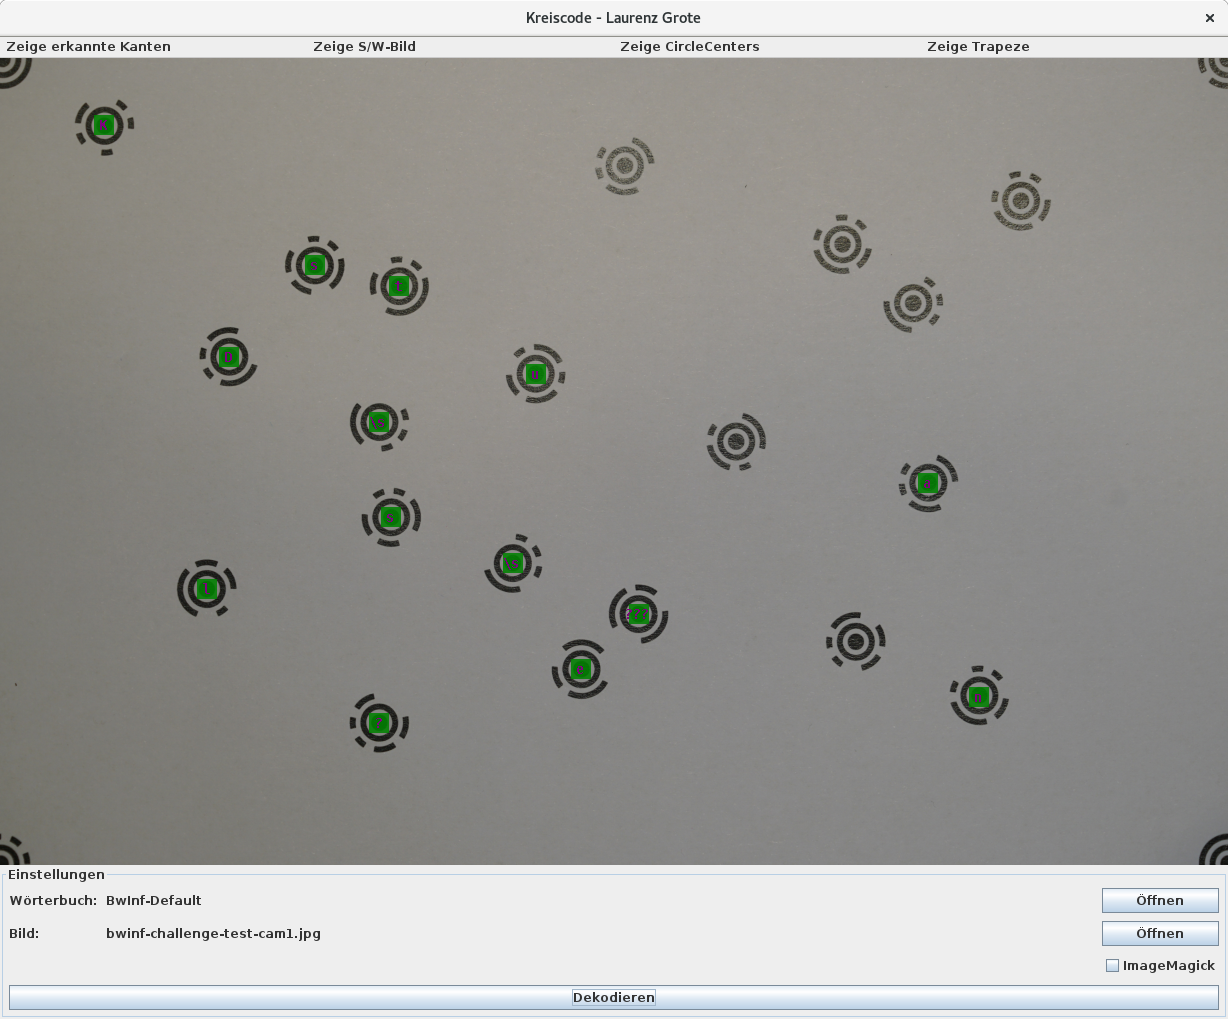
\includegraphics[width=0.9\textwidth]{Grafiken/Ausgaben/cam1}
\includegraphics[width=0.9\textwidth]{Grafiken/Ausgaben/cam4}
\end{minipage}
\begin{minipage}{0.3\textwidth}
Hier scheitert mein Algorithmus an den zahlreichen weißen Punkten in den nicht erkannten Kreis-Codes. Eine stärkere Weichzeichnung ist nicht zielführend, da dann die Kantengrenzen verwischen. Ein geringerer Schwellwert sorgt für False Positives an den Farbwechseln.
\end{minipage}

\subsubsection{Beispiel 8}
\begin{minipage}{0.7\textwidth}
\includegraphics[width=0.9\textwidth]{Grafiken/Ausgaben/cam8}
\end{minipage}
\begin{minipage}{0.3\textwidth}
In diesem Bild sind die Kreise so unscharf, dass eine Erkennung der Kanten bei einigen Kreisringen fehlschlägt
\end{minipage}

\subsubsection{Beispiel B}
\begin{minipage}{0.7\textwidth}
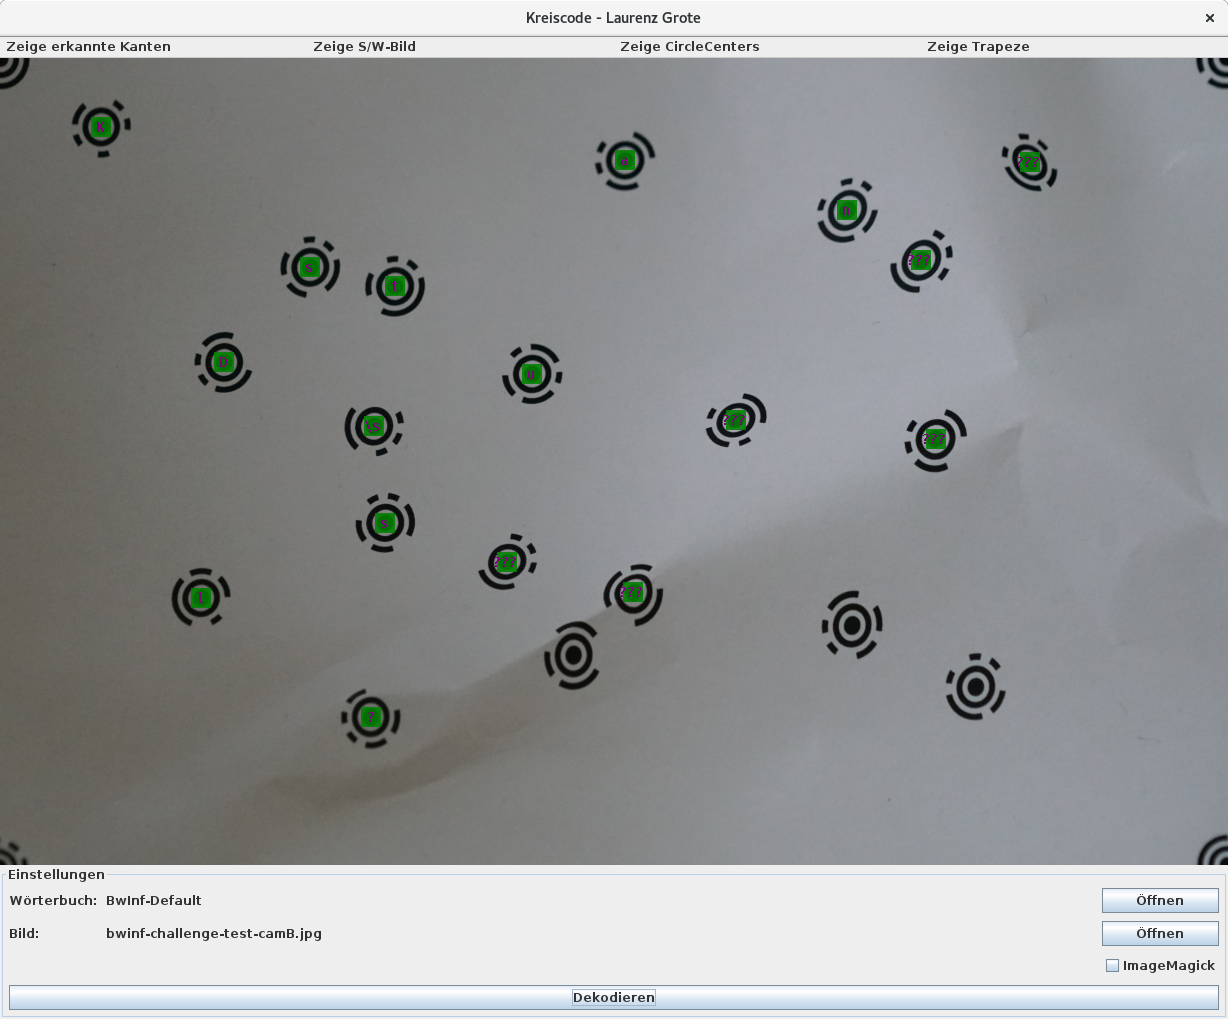
\includegraphics[width=0.9\textwidth]{Grafiken/Ausgaben/camB}
\end{minipage}
\begin{minipage}{0.3\textwidth}
In der oberen rechten Hälfte ist das Blatt geknickt worden. Da in meinem Algorithmus keinerlei Maßnahmen zur Begradigung eingebaut sind, kann der Kreis-Code nicht entziffert werden, da die Trapeze nicht auf den Kreisringsegmenten liegen. Auch nach einer Internetrecherche habe ich keinen Algorithmus gefunden, der dieses Problem ohne eine gerade Referenz behebt.
\end{minipage}

\pagebreak
\section{Eigene Beispiele}
In meinen Beispielen habe ich typische Use-Cases von Barcodes evaluiert. Zum einen habe ich Kreis-Codes in ein Textdokument (blatt.png) eingebettet, da insbesondere QR-Codes oft genutzt werden, um z.B. Links anzugeben.
Auch habe ich einen Kreiscode an meine Zimmerwand geheftet. Damit zeige ich, dass die Bildumrandung nicht zwingend Weiß sein muss, sondern auch sonstige ruhige Flächen wie Raufasertapeten ein geeignete Träger für einen Kreis-Code sind.
Zuguterletzt habe ich ein Bild mit roten Kreis-Codes erstellt. Oftmals möchten Nutzer Barcodes kreativ personalisieren, damit sie besser in ihre Umgebung passen.

\begin{center}
\includegraphics[width=0.4\textwidth]{Grafiken/Ausgaben/blatt}
\hspace{1em}
\includegraphics[width=0.4\textwidth]{Grafiken/Ausgaben/farbig}
\end{center}
\begin{center}
\includegraphics[width=0.8\textwidth]{Grafiken/Ausgaben/raufaser}
\end{center}

\section {Operationsbereich des Programmes}
Mit den Erfahrungen aus den BwInf-Beispielen und eigenen Testfällen habe ich untersucht, welche Voraussetzungen gegeben sein müssen, damit die Dekodierung erfolgreich ist:
\begin{itemize}
	\item Der Hintergrund muss eine ruhige, zusammenhängende Fläche sein. Sonst gelingt die Flood-Fill zur Hintergrundmarkierung nicht. Wenn beispielsweise das Blatt Papier auf eine schwarze Unterlage gelegt wird, ist das gesamte Blattinnere invertiert, da die Außenkante des Blattes als Kante eines Kreis-Codes aufgefasst wird. Ruhig bedeutet in diesem Zusammenhang, dass Farben sanft ineinander verlaufen müssen.
	\item Der Sobel-Operator muss an mindestens einer Stelle jeder Linie des Kreis-Codes einen Wert höher als 40 liefern. Sonst wird diese Kante nicht verfolgt. Die Farbe des Kreis-Codes ist beliebig, es muss nur der Kontrast zum Hintergrund hinreichend groß sein.
	\item Das Blatt darf nicht zerknickt oder zerknüllt sein, die Kamera muss senkrecht auf den Kreis-Code zeigen. Schließlich basieren die Formeln für den Trapezkranz auf der Annahme, das das Bild glatt vorliegt. 
	\item Das Rauschen des Kamerabildes darf nicht zu groß sein. Ein Rauschen wie in Bild Noise-50 entsteht allerdings nur in stark verstrahlten Gebieten oder GIMP, daher ist die Entrauschung meines Programms für Alltagssituationen ausreichend.
\end{itemize}